\pdfminorversion=4
\documentclass[a4paper,12pt]{article}
\usepackage [spanish]{babel} 
\usepackage[utf8]{inputenc}
\usepackage{amsmath}
\usepackage{graphicx}
\usepackage{framed}

\usepackage{fancyhdr}

\newcommand{\ihat}{\hat{\textbf{\i}}}
\newcommand{\jhat}{\hat{\textbf{\j}}}
\newcommand{\khat}{\hat{\textbf{k}}}
\newcommand{\vol}{\mathop{\ooalign{\hfil$V$\hfil\cr\kern0.08em--\hfil\cr}}\nolimits}

\graphicspath{{../img/}}
 
\pagestyle{fancy}
\setlength\headheight{1.5cm}
\fancyhf{}
\rhead{\includegraphics[width=3.0cm]{logo-mec.png}}
\lhead{\includegraphics[width=3.5cm]{logo-utfsm.png}}
\renewcommand{\footrulewidth}{0.5pt}
\rfoot{\tiny{Departamento de Ingenier\'ia Mec\'anica}}
\lfoot{\tiny{Universidad T\'ecnica Federico Santa Mar\'ia}}

\title{Clase 03 --- Flujo potencial: Laplace y flujos elementales} 
\author{Christopher Cooper}
\date{}

\begin{document}
\maketitle
\begin{framed}

Objetivos:
\begin{itemize}
    \item Estudiar las propiedades de la ecuación de Laplace. 
    \item Presentar flujos potenciales elementales. 
\end{itemize}

Contenidos:
\begin{itemize}
    \item Repaso de flujos ideales.
    \item Condiciones de contorno para la ecuación de Laplace.
    \item Flujos potenciales elementales.
\end{itemize}

Bibliografía:
\begin{itemize}
    \item White, F. M. (2008) Mecánica de Fluidos. McGraw-Hill. Sexta edición. Secciones 4.9-4.10
    \item Fox, R. W., Pritchard, P. J. y McDonald, A. T. (2009) Introduction to Fluid Mechanics. John Wiley \& Sons. Sección 6.7.
\end{itemize}
\end{framed}

\section*{Flujo potencial}
La clase pasada introducimos un par de conceptos nuevos, al menos en el contexto de mecánica de fluidos: la función corriente ($\psi$) y la función potencial ($\phi$). 
Un campo de velocidad tiene una función corriente cuando éste tiene divergencia nula y bidimensional, y tiene una función potencial cuando es irrotacional, donde
%
\begin{align}\label{eq:phi_def_3}
u &= \frac{\partial\phi}{\partial x} = \frac{\partial\psi}{\partial y}\nonumber\\
v &= \frac{\partial\phi}{\partial y} = -\frac{\partial\psi}{\partial x}
\end{align}
%
Físicamente, esto significa que el flujo debe ser incompresible y no viscoso, o sea, un \emph{flujo ideal}.

En la vida real, no exiten los flujos totalmente ideales, pero hay ciertas situaciones en que se comportan muy cercano a ideal y la teoría de flujo potencial nos ayuda a modelarlos.
Dos ejemplos son
\begin{itemize}
\item Flujo sobre cuerpos sumergidos, lejos de cuerpo: muy aplicado a aerodinámica, que revisaremos en un par de clases más. El flujo se ve afectado cerca del cuerpo, pero si uno se aleja de este, el flujo es prácticamente potencial.
\item Tornados: el flujo atmosférico de escala ``global'' puede ser visto como bidimiensional, ya que la dimensión de altura es muchísimo más chica que la extensión en los otros sentidos. Un tornado se aproxima muy bien por un vórtice ideal.
\end{itemize}

Además, vimos que al haber una función potencial de la velocidad y que el flujo sea incompresible ($\nabla\cdot\mathbf{V}=0$), el potencial $\phi$ debe satisfacer la ecuación de Laplace
%
\begin{equation}\label{eq:pot_laplace}
\nabla^2\phi = \frac{\partial^2 \phi}{\partial x^2} + \frac{\partial^2 \phi}{\partial y^2} = 0.
\end{equation}

Ya vimos la clase pasada que la línea que define $\psi=$constante corresponde a una línea de flujo \mbox{?`}Cómo es el caso para $\phi=$constante?
Consideremos la curva $y=y(x)$ que describe $\phi(x,y(x))=$constante, y derivemos esto en función de $x$:
%
\begin{align}\label{eq:linea_potencial}
\frac{d\phi}{dx} &= \frac{\partial\phi}{\partial x}\frac{dx}{dx} + \frac{\partial\phi}{\partial y} \frac{dy}{dx} = 0\nonumber\\
\Rightarrow &\frac{dy}{dx} = \frac{\partial\phi/\partial x}{\partial\phi/\partial y} = \frac{u}{v}.
\end{align}
%
La clase pasada dijimos que en una línea de flujo $dy/dx=v/u$, lo cual es exactamente perpendicular al resultados que llegamos en la Ec. \eqref{eq:linea_potencial}.
Por lo tanto, las líneas de $\phi=$constante son perpendiculares a las líneas de $\psi=$constante.

\subsection*{Condiciones de contorno}
Para resolver una ecuación diferencial necesitamos condiciones de contorno y/o iniciales.
En el caso de mecánica de fluidos, las condiciones de contorno están relacionadas con la velocidad, ya sea en el contacto del fluido con un sólido, como en la interfaz entre dos fluidos, o en regiones lejos de cualquier perturbación. 
Necesitamos entonces traducir esas condiciones de contorno de velocidad, que son muy intuitivas, a potencial $\phi$. 
Veámoslo caso a caso:
%
\begin{itemize}
\item \emph{Superficie sólida:} ya sabemos que en el caso de un flujo viscoso, la viscosidad fuerza al fluido a tener la misma velocidad que la pared sólida en la interfaz (no deslizamiento). 
En este caso, el flujo no es viscoso y no se cumple la condición de no deslizamiento, sin embargo, el fluido no puede penetrar la pared (condición de impermeabilidad).
Esto significa que en la pared, la componente de la velocidad normal a la superficie debe ser cero:
%
\begin{equation}
\mathbf{V}_\mathbf{n} = 0
\end{equation}
%
donde $\mathbf{n}$ es un vector unitario normal a la superficie.
Usando la Ec. \eqref{eq:phi_def_3}, vemos que en términos de $\phi$, esto es:
%
\begin{equation}\label{eq:phi_pared_bc}
\nabla\phi\cdot\mathbf{n} = \frac{\partial\phi}{\partial\mathbf{n}} = 0.
\end{equation}
%
La Ec. \eqref{eq:phi_pared_bc} es una condición de borde de Neumann que dice que la variación de $\phi$ normal a la superficie debe ser cero.
Noten que si a la condición de borde en la Ec. \eqref{eq:phi_pared_bc} le agregamos que $\mathbf{V}\cdot\mathbf{t}$ donde $\mathbf{t}$ es un vector tangencial a la superficie, llegamos a la condición de borde de no deslizamiento.

\item \emph{Interfaz entre dos fluidos:} si tenemos dos fluidos no viscosos, ellos van a ser capaces de deslizarse en la interfaz.
Sin embargo, la componente normal de la velocidad en la interfaz debe ser la misma, ya que si no, se podrían crear ``hoyos'' sin fluido!
%
\begin{equation}
\mathbf{V}_1\cdot\mathbf{n}=\mathbf{V}_2\cdot\mathbf{n},
\end{equation}
%
donde $1$ y $2$ denotan los dos fluidos, y $\mathbf{n}$ es un vector normal a la interfaz.
En términos de $\phi$, queda
%
\begin{equation}
\frac{\partial\phi_1}{\partial\mathbf{n}} = \frac{\partial\phi_2}{\partial\mathbf{n}}
\end{equation}

\item \emph{Flujo al infinito:} la teoría de flujo potencial se muy usado para modelar flujos al infinito, por ejemplo, cuerpos sumergidos.
De hecho, en este caso podemos derivar una condición de contorno muy intuitiva: el flujo que se encuentra muy lejos de un cuerpo sumergido no debiese sentir su presencia.
Por lo tanto, si el fluido se aproxima con una velocidad $\mathbf{V}=\mathbf{V}_\infty$, podemos decir que
%
\begin{align}
\mathbf{V}_{r\to\infty}=&\mathbf{V}_\infty\text{, o, }\nonumber\\
\nabla\phi(r\to\infty) =&\mathbf{V}_\infty 
\end{align}
\end{itemize}

%\section*{Propiedades de la ecuación de Laplace}
%La Ec. \eqref{eq:pot_laplace} se conoce como ecuación de Laplace.
%Ésta es la ecuación diferencial parcial más simple que podemos encontrar, sin embargo, es muy útil en la modelación de muchos fenómenos físicos: electrostática, conducción de calor, flujo potencial, etc.

\section*{Flujos planos elementales}
No haremos la demostración acá, pues es más un tema de matemática pura, pero la ecuación de Laplace para un set definido de condiciones de contorno tiene solución única
\mbox{?`}Qué significa esto para nosotros?
Que si tenemos una situación donde enforzamos algunas de las condiciones de borde que discutimos en la sección anterior, el resultado de la ecuación de Laplace va a ser único y éste tendrá sentido físico (en el contexto de que consideramos un flujo no viscoso e incompresible como ``físico'').
Esto nos entrega una poderosa herramienta de modelación, ya que la ecuación de Laplace es muchísimo más simple que la de Navier-Stokes, y representa un buen modelo para flujos en que la viscosidad y la compresibilidad no juega un rol importante.

Existe un grupo de flujos que llamamos ``elementales'' que no son más que soluciones de la ecuación de Laplace en la Ec. \eqref{eq:phi_def_3} con condiciones de contorno físicas.
A partir de éstas, se hacen estudios muy elaborados en, por ejemplo, aerodinámica.
Sin embargo, no son las únicas formas de flujo potencial: mientras la función sea solución de la ecuación de Laplace y cumpla con condiciones de borde físicas, ésta perfectamente puede representar a un flujo.

\subsection*{Flujo uniforme}
La ecuación de Laplace involucra segundas derivadas igualadas a cero
\mbox{?`}Cuál es la función más simple que pueden pensar que cumple con esa condición? Una función lineal ($\phi=Ax$).
Agreguémosles a esto condiciones de contorno físicas: la velocidad al infinito es uniforme y horizontal $\mathbf{V}_{r\to\infty}=\partial\phi/\partial x=U_\infty\ihat$.
El resultado es un flujo uniforme horizontal con velocidad $U_\infty$, como el que muestra la Figura \ref{fig:flujo_uniforme}.
%
\begin{figure}[!h]
\centering
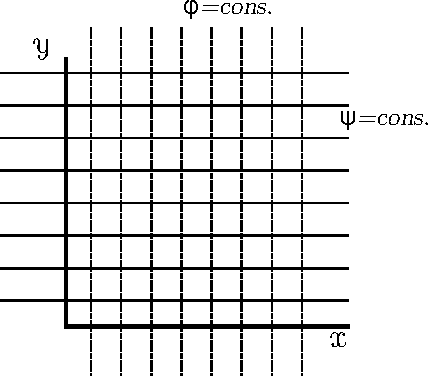
\includegraphics[width=0.7\textwidth]{clase03/flujo_uniforme.pdf}
\caption{Flujo uniforme eje x}
\label{fig:flujo_uniforme}
\end{figure}

En la Figura \ref{fig:flujo_uniforme} el flujo se mueve horizontalmente, de izquierda a derecha, con velocidad $U_\infty$.
La ecuación del potencial es $\phi=U_\infty x$, por lo que las líneas de $\phi$ constante son líneas de $x$ constante, o sea, paralelas al eje $y$.
Por otra parte, las líneas de flujo ($\psi$ constante) deben ser perpendiculares a las líneas de equipotencial.
Chequémos esto:
%
\begin{align}
\frac{\partial\psi}{\partial y} &= u = U_\infty \Rightarrow \psi=U_\infty y + f(x) \nonumber \\
\frac{\partial\psi}{\partial x} &= \frac{\partial}{\partial x}\left(U_\infty y + f(x)\right) = f'(x) = -v = 0 \Rightarrow f(x) = C_0 = 0.
\end{align}
%
La líneas de $\psi$ constante son líneas de $y$ constante, paralelas al eje $x$, confirmando que son perpendiculares a las líneas de equipotencial.

Podemos hacer el mismo trabajo en casos parecidos.
Por ejemplo, el flujo en dirección vertical con velocidad $V_\infty$ se obtiene con $\phi=V_\infty y$, y la solución es igual a la Figura \ref{fig:flujo_uniforme}, pero con las líneas de $\phi$ y $\psi$ constante intercambiadas.
Otro caso: \mbox{?`}cómo obtener un flujo en la dirección contraria? Simplemente cambiando de signo las condiciones de borde ($-U_\infty$ o $-V_\infty$).

En resumen:
%
\begin{itemize}
\item Flujo uniforme horizontal
\begin{align}
u &= U_\infty \quad v = 0 \nonumber \\
\phi&=\pm U_\infty x \quad \psi= \pm U_\infty y
\end{align}

\item Flujo uniforme vertical
\begin{align}
u &= 0 \quad v = V_\infty \nonumber \\
\phi&=\pm V_\infty y \quad \psi= \mp V_\infty x
\end{align}
%
Noten que $\pm$ y $\mp$ están dados vuelta en el último caso, debido al signo negativo en la última expresión de $\psi$ en la Ec. \eqref{eq:phi_def_3}.
\end{itemize}

\subsection*{Fuente y sumidero}
El siguiente caso simple tiene una derivación algo más complicada, pero vale la pena hacerla porque la encontramos en muchas aplicaciones físicas (electromagnetismo, acústica, entre otras).
Digamos que queremos resolver la siguiente ecuación, con condición de borde de velocidad cero al infinito:
%
\begin{align}\label{eq:fuente_laplace}
\nabla^2\phi=q\delta(r)\nonumber\\
\mathbf{V}(r\to\infty)=\nabla\phi(r\to\infty) = 0,
\end{align}
%
donde $q$ es una constante y $\delta(r)$ se conoce como la función \emph{delta de Dirac}:
%
\begin{equation}
\delta(r) = 
\begin{cases}
\infty \text{ si } r=0,\\
0 \text{ en otro caso.}
\end{cases}
\end{equation}
%
Ustedes debiesen conocer la función $\delta(r)$ de sus clases de matemáticas, pero si no se acuerdan, solamente necesitan saber dos propiedades:
%
\begin{align}\label{eq:prop_delta}
\int_{\vol} \delta(\mathbf{r}-\mathbf{r}_0)d\mathbf{r}=&
\begin{cases}
1 \text{ si $\mathbf{r}_0$ está dentro del volumen $\vol$}\\
0 \text{ si $\mathbf{r}_0$ está fuera de $\vol$}
\end{cases}\nonumber\\
\int_{\vol} f(\mathbf{r}) \delta(\mathbf{r}-\mathbf{r}_0)d\mathbf{r}=&
\begin{cases}
f(\mathbf{r}_0) \text{ si $\mathbf{r}_0$ está dentro del volumen $\vol$}\\
0 \text{ si $\mathbf{r}_0$ está fuera de $\vol$.}
\end{cases}
\end{align}
%
En palabras, si el dominio de la integral pasa por el punto donde $delta$ está centrado ($\mathbf{r}_0$), su integral es $1$ y si está multiplicando a una función cualquiera, el resultado de la integral es la función evaluada en ($\mathbf{r}_0$).
Si la integral no pasa por $\mathbf{r}_0$, todo da cero.

Al mirar la Ec. \eqref{eq:fuente_laplace}, lo primero que salta a la vista es que no hay un cero a la derecha \mbox{!`}no es la ecuación de Laplace!
Pero $\delta$ es diferente a cero solamente en el origen ($r=0$), por lo que para $r>0$ la Ec. \eqref{eq:fuente_laplace} si es la ecuación de Laplace.

Veamos la Ec. \eqref{eq:fuente_laplace} de cerca para responder dos cosas {\bf(1)} \mbox{?`}Qué significa la constante $q$? y {\bf(2)} \mbox{?`}Cuál es la solución de la ecuación?

\paragraph{El significado físico de $q$}
Agarremos la Ec. \eqref{eq:fuente_laplace} e integrémosla en un dominio $\vol$ que incluya el origen, donde $\delta$ está ubicado:
%
\begin{equation}
\int_{\vol}\nabla^2\phi d\mathbf{r}= \int_{\vol}q\delta d\mathbf{r}. 
\end{equation}
%
La integral a la derecha es fácilmente resolvible con las propiedades de la Ec. \eqref{eq:prop_delta}, y a la de la izquierda se le puede aplicar el teorema de la divergencia:
%
\begin{equation}\label{eq:fuente_int}
\int_{\partial\vol}\nabla\phi\cdot\mathbf{n}dS = q,
\end{equation}
%
donde $\partial\vol$ es la frontera de $\vol$, $dS$ un elemento diferencial de $\vol$, y $\mathbf{n}$ es un vector unitario normal a $\partial\vol$.
Pero $\nabla\phi=\mathbf{V}$, por lo que obtenemos
%
\begin{equation}
\int_{\partial\vol}\mathbf{V}\cdot\mathbf{n}dS = q,
\end{equation}
%
y lo que tenemos en el lado izquierdo de la ecuación no es más que la definición de caudal que pasa por la superficie $\partial\vol$, dándole un sentido físico a la constante $q$..
Todavía no hemos definido la superficie $\partial\vol$, y solamente hemos dicho que encierra al origen, por lo que sería perfectamente válido que fuera un círculo con un radio muy muy pequeño centrado en el origen \mbox{?`}de dónde sale el caudal $q$?
Como $q\neq0$, dentro del volumen $\vol$ tiene que haber algo que esté generando (o sacando) flujo: la función $\delta$ es una fuente (o sumidero) de fluido.

\paragraph{Solución de $\phi$}
En coordenadas polares, el operador Laplaciano es 
%
\begin{equation}
\nabla^2\phi = \frac{1}{r}\frac{\partial\phi}{\partial r} + \frac{\partial^2\phi}{\partial r^2} + \frac{1}{r^2}\frac{\partial^2\phi}{\partial\theta}.
\end{equation}
%
y considerando solamente un flujo radial, la Ec. \eqref{eq:fuente_laplace} en el dominio $r>0$ es
%
\begin{equation}
\frac{1}{r}\frac{\partial\phi}{\partial r} + \frac{\partial^2\phi}{\partial r^2} = 0.
\end{equation}
%
Considerando la condición de contorno $\nabla\phi(r\to\infty)=0$, por inspección podemos llegar a que la solución tiene la forma 
%
\begin{equation}
\phi = A_0\ln(r) + B_0,
\end{equation}
%
y necesitamos saber el valor de $A_0$ (por simplicidad, asumiremos $B_0=0$).
Revisitemos la Ec. \eqref{eq:fuente_int} conociendo la solución para $\phi$ que propusimos recién.
Para hacernos la vida más fácil, consideremos que $\vol$ es un círculo de radio $R$, ya que así la componente $r$ y el vector normal $\mathbf{n}$ están alineados, y no nos molesta el producto punto.
Sabiendo que $\nabla\phi=\partial\phi/\partial r$, llegamos a que
%
\begin{align}
\int_{\partial\vol}\frac{\partial(A\ln(r))}{\partial{r}}dS &= q\nonumber\\
\frac{A_0}{R}2\pi R&= q\nonumber\\
\Rightarrow A_0 &= \frac{q}{2\pi}.
\end{align}
%
Así llegamos a que
\begin{equation}
\phi=\frac{q}{2\pi}\ln(r)\nonumber\\
\end{equation}

Esta última ecuación se conoce como función de Green para el operador laplaciano en dos dimensiones. 
La función de Green es tremendamente útil en muchas aplicaciones: electroestática, electrodinámica, acústica, y un largo etc. y de ahí lo interesante de que vean de donde viene.
De hecho, probablemente ya la han usado sin darse cuenta.
En tres dimensiones, la función de Green es $\frac{1}{r}$ \mbox{?`}se acuerdan del potencial electrostático de una carga puntual? Es exactamente el mismo concepto.
De hecho, si cambiamos $\mathbf{V}$ por el campo eléctrico $\mathbf{E}$, todo lo que hemos visto se aplica a electrostática.
Otro ejemplo más cercano a la mecánica: el $\frac{1}{r}$ del potencial gravitacional de planetas aparece al modelar planetas como masas puntuales en el espacio, y se modela con la ecuación de Laplace.

En coordenadas polares, la gradiente se define como $\nabla()=(\partial()/\partial r,1/r\partial()/\partial\theta)$, donde la primera componente es radial y la segunda angular.
Sabiendo que $\nabla\phi=\mathbf{V}=(V_r,V_\theta)$:
%
\begin{equation}\label{eq:Vfuente}
V_r = \frac{\partial\phi}{\partial r} = \frac{q}{2\pi r}\quad V_\theta= \frac{1}{r}\frac{\partial\phi}{\partial\theta}=0.
\end{equation}
%
Esto nos dice que la solución ecuación diferencial en \eqref{eq:fuente_laplace} es un flujo radial, con una fuente en el centro, donde su velocidad decae a medida que nos alejamos del centro.

Por otra parte, sabemos que las líneas de corriente ($\psi=$constante) son perpendiculares a la líneas de equipotencial, así es que podemos escribir $\psi$ intercambiando $V_r$ y $V_\theta$:
\begin{equation}\label{eq:psi_polar}
V_r=\frac{1}{r}\frac{\partial\psi}{\partial\theta} \quad V_\theta=-\frac{\partial\psi}{\partial r}
\end{equation}

Insertando la expresión de $V_r$ en la Ec. \eqref{eq:Vfuente} en la Ec. \eqref{eq:psi_polar} e integrando, llegamos a que
%
\begin{equation}
\psi = \int V_rr d\theta = \int\frac{q}{2\pi r} rd\theta = \frac{q}{2\pi}\theta. 
\end{equation}

En resumen:
\begin{itemize}
\item Fuente:
\begin{align}
V_r &= \frac{q}{2\pi r}\quad V_\theta=0\nonumber\\
\phi&=\frac{q}{2\pi}\ln(r) \quad \psi=\frac{q}{2\pi}\theta
\end{align}
\item Sumidero:
\begin{align}
V_r &= -\frac{q}{2\pi r}\quad V_\theta=0\nonumber\\
\phi&=-\frac{q}{2\pi}\ln(r) \quad \psi=-\frac{q}{2\pi}\theta
\end{align}
\end{itemize}
%
y el flujo se muestra en la Figura \ref{fig:fuente}
%
\begin{figure}[h!]
\centering
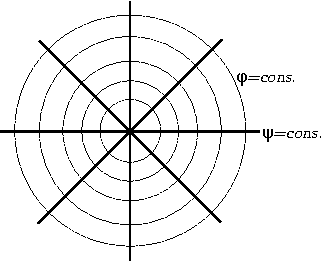
\includegraphics[width=0.7\textwidth]{clase03/fuente.pdf}
\caption{Fuente o sumidero.}
\label{fig:fuente}
\end{figure}

En la Figura \ref{fig:fuente} se ve que las líneas de flujo son de $\theta=$constante y las de equipotencial de $r=$constante.

\subsection*{Vórtice}
Demos vuelta un poco las cosas.
Acabamos de resolver la ecuación $\nabla^2\phi=\delta$, y vimos que las líneas de equipotencial eran circulares (Figura \ref{fig:fuente}).
Tratemos de generar un flujo donde las líneas de flujo sean las circulares: reemplacemos $\phi$ por $\psi$ en la Ec. \eqref{eq:fuente_laplace}
%
\begin{align}\label{eq:lap_psi}
\nabla^2\psi=\Gamma\delta(r)\nonumber\\
\mathbf{V}(r\to\infty)=0.
\end{align}
%
Donde $\Gamma$ es, por ahora, solamente una constante.
\mbox{?`}Tiene algún sentido lo que estamos haciendo? La respuesta es si.
Ya vimos la clase pasada que $\nabla^2\psi=\omega_z$, por lo que la Ec. \eqref{eq:lap_psi} es una distribución tipo ``delta'' de la vorticidad, y el flujo sigue siendo irrotacional (y potencial o ideal) para $r>0$.

No es necesario repetir todo lo que hicimos anteriormente, sabemos que la solución es 
%
\begin{align}
\phi&=\frac{\Gamma}{2\pi}\theta \nonumber\\
\Rightarrow V_r &= 0 \quad V_\theta=\frac{\Gamma}{2\pi r}\nonumber\\
\Rightarrow \psi &= -\int V_\theta dr = -\frac{\Gamma}{2\pi}\ln(r)
\end{align}
%
Este flujo se llama vórtice, donde la velocidad es angular y su magnitud va decayendo a medida que nos alejamos del centro del vórtice.
Este tipo de flujos es muy útil para modelar, por ejemplo, tornados, que se comportan como flujo potencial alejados de su centro.

Gráficamente, el vórtice es igual a la Figura \ref{fig:fuente}, pero con las líneas de corriente y equipotenciales intercambiadas, como aparece en la Figura \ref{fig:vortice}.

\begin{figure}[h!]
\centering
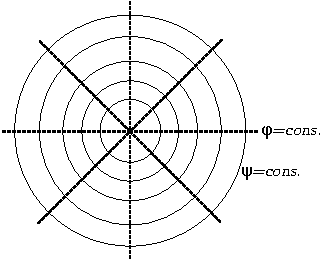
\includegraphics[width=0.7\textwidth]{clase03/vortice.pdf}
\caption{Vórtice.}
\label{fig:vortice}
\end{figure}

La pregunta es, así como encontramos que $q$ era el caudal que salía de la fuente (o se iba por el sumidero) \mbox{?`}Cuál es el significado físico de $\Gamma$?
Ya discutimos que el lado derecho de la Ec. \eqref{eq:lap_psi} es una distribución puntual de vorticidad ($\Gamma\delta=\omega_z$).
Si integramos esto en todo el espacio, y viendo las propiedades en la Ec. \eqref{eq:prop_delta}, llegamos a
%
\begin{align}
\int\Gamma\delta d\mathbf{r} &= \int\omega_z d\mathbf{r}\nonumber\\
\Gamma &= \int\omega_z d\mathbf{r},
\end{align}
%
lo cual es la definición de circulación que discutimos la clase pasada.
$\Gamma$ es la circulación.

\subsection*{Doblete}
Por último, el doblete aparece de la superposición de una fuente y un sumidero de igual $q$ que están infinitesimalmente cerca en el origen.
Para esta derivación, necesitaremos saber como expresar una fuente y sumidero que no están ubicados en el centro, y luego veremos como se comporta esa solución a medida que los acercamos al límite en que la distancia entre ellos tiende a cero.
%
\begin{figure}[!h]
\centering
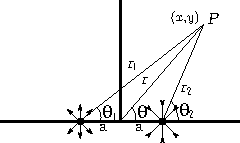
\includegraphics[width=0.7\textwidth]{clase03/fuente_sumidero.pdf}
\caption{Fuente y sumidero a distancia $a$ del centro.}
\label{fig:fuente_sumidero}
\end{figure}

La función corriente de la fuente es $\psi_f=\frac{q}{2\pi}\theta_1$ y el del sumidero $\psi_s=-\frac{q}{2\pi}\theta_2$, por lo tanto, la función corriente del doblete es la suma de estas dos contribuciones $\psi=\frac{q}{2\pi}(\theta_1-\theta_2)$.
El punto $P$ en la Figura \ref{fig:fuente_sumidero} está ubicado en el punto $(x,y)$, por lo tanto $\tan(\theta_1)=\frac{y}{x+a}$ y $\tan(\theta_2)=\frac{y}{x-a}$, y usando identidades trigonométricas, podemos decir que
%
\begin{align}
\tan(\theta_1-\theta_2) &= \frac{\tan(\theta_1)-\tan(\theta_2)}{1+\tan(\theta_1)\tan(\theta_2)}\nonumber\\
&=\frac{\frac{y}{x+a}-\frac{y}{x-a}}{1+\frac{y}{x+a}\frac{y}{x-a}} = \frac{y(x-a)-y(x+a)}{x^2-a^2+y^2} = -\frac{2ya}{x^2-a^2+y^2}.
\end{align}
%
Veamos ahora que pasa en el límite en que $a\to0$.
En ese caso, $\theta_1$ es muy cercano a $\theta_2$, y por aproximación de ángulo pequeño $\tan(\theta_1-\theta_2)\approx\theta_1-\theta_2$.
Además, al $a\to0$, $x^2-a^2+y^2\approx x^2+y^2$.
Por otra parte, y para que todo nuestro resultado no se vaya a cero, saquemos el límite $q\to\infty$ para que así $qa$ tienda a un numero finito.
Con todo esto, la suma de la fuente más el sumidero, queda
%
\begin{equation}
\psi=\frac{q}{2\pi}(\theta_1-\theta_2) = -\frac{q}{2\pi}\frac{2ya}{x^2+y^2}.
\end{equation}
%
Llamemos $K=\frac{qa}{\pi}$, y reemplacemos por coordenadas polares ($y=r\sin\theta$, $r=\sqrt{x^2=y^2})$:
%
\begin{equation}
\psi = -K\frac{r\sin(\theta)}{r^2}=-K\frac{\sin(\theta)}{r}.
\end{equation}

Usando la Ec. \eqref{eq:psi_polar}, llegamos a
%
\begin{equation}
V_r = -K\frac{\cos(\theta)}{r^2}\quad V_\theta = -K\frac{\sin(\theta)}{r^2}
\end{equation}
%
e integrando estas expresiones, encontramos el potencial $\phi$:
%
\begin{equation}
\phi=K\frac{\cos(\theta)}{r}
\end{equation}
%
La Figura \ref{fig:doblete} muestra las líneas de corriente y equipotenciales de un doblete.
%
\begin{figure}[h!]
\centering
\includegraphics[width=0.7\textwidth]{clase03/doblete_2.jpeg}
\caption{Doblete}
\label{fig:doblete}
\end{figure}

 
\end{document}
